\chapter{EG-X Model}\label{ch:eg-x-model}

\section{Lattice Structure of Graphene}\label{sec:lattice-structure-of-graphene}

Following~\cite{Yang_Li_Lee_Ng_2018}.

Monolayer graphene forms a hexagonal lattice.
This is formed by two triangular sub lattices.
So in the unit cell of the hexagonal actually has two atoms.

Primitive lattice vectors of the hexagonal lattice:
\begin{align}
    \vb{a}_1 &= \frac{a_0}{2} \begin{pmatrix} 3 \\ \sqrt{3} \end{pmatrix} \\
    \vb{a}_2 &= \frac{a_0}{2} \begin{pmatrix} 3 \\ -\sqrt{3} \end{pmatrix} \\
\end{align}
with \(a_0 = \SI{1.42}{\angstrom}\) the distance between nearest neighbours.

Vectors to the nearest-neighbor \(B_l\) (\(l = 1, 2, 3,\)) from atom \(A_i\):
\begin{align}
    \vb{\updelta} =
\end{align}


\section{EG-X Model}\label{sec:eg-x-model}

Graphene lattice and a site X\@.
Real-life motivation: layer of graphene on top of a substrate of another material (which provides the additional X atoms).

Without interaction:
\begin{equation}
    H_0 = -t_{\mathrm{X}} \sum_{\langle ij \rangle, \sigma \sigma^{\prime}} d_{i, \sigma}^{\dagger} d_{j, \sigma^{\prime}}
    -t_{\mathrm{Gr}} \sum_{\langle ij \rangle, \sigma \sigma^{\prime}} \left(
    c_{i, \sigma}^{(A), \dagger} c_{j, \sigma^{\prime}}^{(B)} +
    c_{j, \sigma^{\prime}}^{(B), \dagger} c_{i, \sigma}^{(A)}
    \right)
    + V \sum_{i, \sigma \sigma^{\prime}} \left(
    d_{i, \sigma}^{\dagger} c_{i, \sigma^{\prime}}^{(A)} +
    c_{i, \sigma}^{(A), \dagger} d_{i, \sigma^{\prime}}
    \right)
    \label{eq:EG-X model Hamiltonian non-interacting}
\end{equation}
with:
\begin{itemize}
    \item \(d\) operators on the X atom
    \item \(c^{(\epsilon)}\) operators on the graphene site (\(\epsilon = A, B\))
    \item \(t_X\) NN hopping for X
    \item \(t_{Gr}\) NN hopping of Gr
    \item \(V\) hybridization between \(\mathrm{X}\) and Graphene \(\mathrm{B}\) sites
\end{itemize}
We can also introduce an onsite Hubbard interaction:
\begin{equation}
    H_{\mathrm{int}} = U_{\mathrm{X}} \sum_{i} d_{i, \uparrow}^{\dagger} d_{i, \downarrow}^{\dagger} d_{i, \downarrow} d_{i, \uparrow}
    + U_{\mathrm{Gr}} \sum_{i, \epsilon=A, B} c_{i, \uparrow}^{(\epsilon) \dagger} c_{i, \downarrow}^{(\epsilon) \dagger} c_{i, \downarrow}^{\epsilon} c_{i, \uparrow}^{\epsilon}
\end{equation}

\subsection{Band structure of the non-interacting EG-X model}\label{subsec:band-structure-of-the-non-interacting-eg-x-model}

To treat eq.~\ref{eq:EG-X model Hamiltonian non-interacting}, we first write out the sums over nearest neighbours \(\langle i, j \rangle\) explicitly, writing \(\vb{\delta}_{\mathrm{X}}, \vb{\delta}_{\epsilon}\) (\(\epsilon = A, B\)) for the connections to the nearest neighbours of the \(\mathrm{X}\) atoms and Graphene \(A, B\) sites.
Doing the calculation for the example of the \(\mathrm{X}\) atoms:
\begin{align}
    -t_{\mathrm{X}} \sum_{\langle ij \rangle, \sigma \sigma^{\prime}} d_{i, \sigma}^{\dagger} d_{j, \sigma^{\prime}}
    &= -\frac{t_X}{2} \sum_{i,\sigma, \sigma^{\prime}} \sum_{\delta_{\mathrm{X}}} d_{i, \sigma}^{\dagger} d_{i + \delta_{\mathrm{X}}, \sigma^{\prime}} \label{eq:EG-X model X atoms nearest neighbours written out} \\
\end{align}
(The factor \(\nicefrac{1}{2}\) is to account for double counting when going to the sum over all lattice sites \(i\))

Now we can input the discrete Fourier transform (for both graphene and X operators) into eq.~\ref{eq:EG-X model X atoms nearest neighbours written out}
\begin{align}
    c_{i} &= \frac{1}{\sqrt{N}} \sum_{\vb{k}} e^{\iu \vb{k} \vb{r}_{i}} c_{\vb{k}} \\
    c_{i}^{\dagger} &= \frac{1}{\sqrt{N}} \sum_{\vb{k}} e^{-\iu \vb{k} \vb{r}_{i}} c_{\vb{k}}^{\dagger}
\end{align}
with the completeness relation:
\begin{equation}
    \sum_{i} e^{\iu \vb{k} \vb{r}_{i}} e^{-\iu \vb{k}^{\prime} \vb{r}_{i}} = N \delta_{\vb{k}, \vb{k}^{\prime}}
    \;.
\end{equation}
We get:
\begin{align}
    -\frac{t_X}{2} \frac{1}{N} \sum_{i,\sigma, \sigma^{\prime}} \sum_{\vb{\delta}_{\mathrm{X}}} d_{i, \sigma}^{\dagger} d_{i + \vb{\delta}_{\mathrm{X}}, \sigma^{\prime}}
    &= -\frac{t_X}{2} \frac{1}{N} \sum_{i,\sigma, \sigma^{\prime}} \sum_{\vb{\delta}_{\mathrm{X}}} \sum_{\vb{k}, \vb{k}^{\prime}} e^{-\iu \vb{k} \vb{r}_i} d_{\vb{k}, \sigma}^{\dagger} e^{\iu \vb{k}^{\prime} \vb{r}_i} e^{\iu \vb{k}^{\prime} \vb{\delta}_{\mathrm{X}}} d_{\vb{k}^{\prime}, \sigma^{\prime}} \\
    &= -\frac{t_X}{2} \frac{1}{N} \sum_{\vb{k}, \vb{k^{\prime}}, \sigma, \sigma^{\prime}} \sum_{\vb{\delta}_{\mathrm{X}}} d_{\vb{k}, \sigma}^{\dagger}  e^{\iu \vb{k}^{\prime} \vb{\delta}_{\mathrm{X}}} d_{\vb{k}^{\prime}, \sigma^{\prime}} \sum_{i} e^{-\iu \vb{k} \vb{r}_i} e^{\iu \vb{k}^{\prime} \vb{r}_i} \\
    &= -\frac{t_X}{2} \frac{1}{N} \sum_{\vb{k}, \vb{k^{\prime}}, \sigma, \sigma^{\prime}} \sum_{\vb{\delta}_{\mathrm{X}}} d_{\vb{k}, \sigma}^{\dagger}  e^{\iu \vb{k}^{\prime} \vb{\delta}_{\mathrm{X}}} d_{\vb{k}^{\prime}, \sigma^{\prime}} N \delta_{\vb{k}, \vb{k}^{\prime}} \\
    &= -\frac{t_X}{2} \sum_{\vb{k}, \sigma, \sigma^{\prime}}  d_{\vb{k}, \sigma}^{\dagger}d_{\vb{k}, \sigma^{\prime}} \sum_{\vb{\delta}_{\mathrm{X}}} e^{\iu \vb{k}^{\prime} \vb{\delta}_{\mathrm{X}}}
\end{align}
Using the expressions for the vectors of neighbouring Graphene atoms from section~\ref{sec:lattice-structure-of-graphene}, we can calculate the so called structural factor \todo{Really called this way?}:
\begin{align}
    \sum_{\vb{\delta}_{\mathrm{X}}} e^{\iu \vb{k}^{\prime} \vb{\delta}_{\mathrm{X}}} &=
\end{align}


\todo{Put matrix formulation here}

Doing the same for the hoppings between the \(A\) and \(B\) Graphene sites as well as the hybridisaton between \(\mathrm{X}\) and Graphene \(A\) lattice sites, we get:
\begin{align}
    H_0 =
\end{align}

The band structure for the non-interacting EG-X model is easily obtained by diagonalising the matrix \todo{reference here!}.
This was done in fig.~\ref{fig:EG-X model non-interacting bands}.

Values used for calculation:
\begin{itemize}
    \item \(t_{\mathrm{Gr}} = 1\)
    \item \(t_{\mathrm{X}} = 0.01\)
\end{itemize}
\(V\) is the control parameter.
(According to Niklas), a range from \(V = 0.1\) to \(V = 2\) can be crudely onto real experimental materials.

\begin{figure}[t]
    \centering
    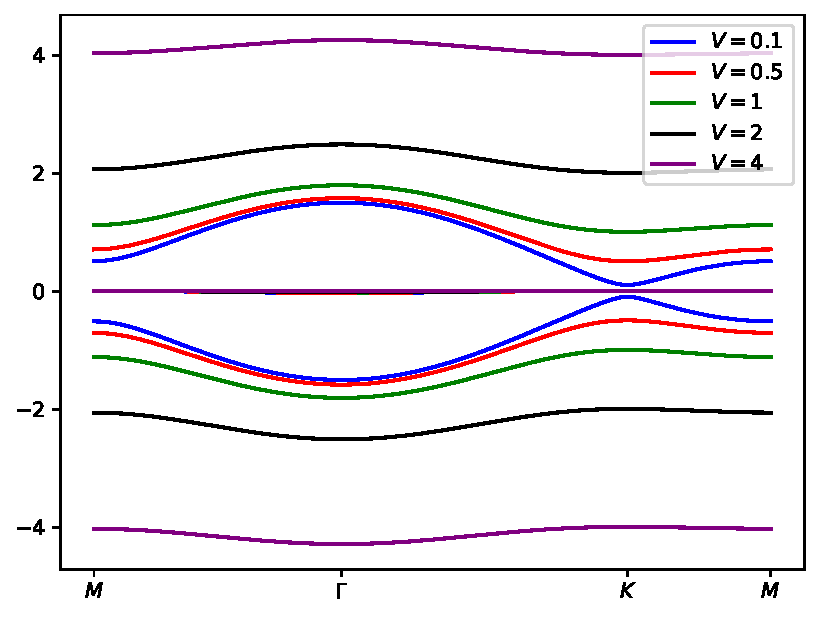
\includegraphics[width=\textwidth]{notes/images/EG_X bands}
    \caption{Bands of the non-interacting EG-X model. All the bands are spin-degenerate.}
    \label{fig:EG-X model non-interacting bands}
\end{figure}

